% Drawing 12/07-1 -- folder 12, batch 07, archive page 136 (PDF page 137).
% Transcription: sous la formule, un croquis du terme $E_{2}$ : trois lignes horizontales, la plus haute marquée « 2 », fermées à droite par un trait vertical marqué « $N$ » ; des points sur les lignes, et deux flèches obliques $d_{2}$ descendant de la ligne 2 vers la ligne 1, puis de la ligne 1 vers la ligne 0, vers la droite
% Kind: sketch of the E_2 term: three rows with d_2 arrows. Method 2 (schematic redraw from the facsimile). Status: ok.
% Notes: Three horizontal lines, the top one marked 2, closed on the left by a vertical stroke and on the right by a vertical stroke; points on the lines and two oblique arrows d_2 going down to the right, from row 2 to row 1 and from row 1 to row 0. The "N" at the right stroke is not visible on the crop; it is placed after the transcription. The labels d_2 are not written beside the arrows on the page.
% Coordinates: 1 unit = 1 mm = 1/100 of the crop width (bbox in page fractions: [0.2, 0.1, 0.55, 0.18]).
% Redrawn by Claude (claude-opus-5-5), issue #73, 2026-11-07; not checked by a human; not compiled (no TeX in the session).
% Rights: reproduces part of the work -- behind RENDER_TRANSCRIPTS, never published by itself.
\documentclass[tikz,border=3pt]{standalone}
\usepackage{amsmath,amssymb}
\usetikzlibrary{patterns,arrows.meta}
\tikzset{pencil/.style={black!45}, struck/.style={black!35}, mark/.style={circle,draw,inner sep=1.3pt}, pt/.style={circle,fill,inner sep=0.9pt}, opt/.style={circle,draw,fill=white,inner sep=1.1pt}}
\begin{document}
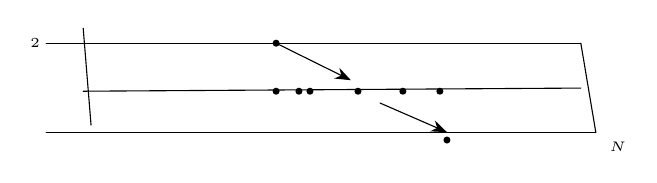
\begin{tikzpicture}[x=1mm,y=1mm,line cap=round,line join=round,font=\scriptsize]
\draw (5.7,-17.9) -- (73.6,-17.9);
\draw (10.4,-24) -- (73.6,-23.6);
\draw (5.7,-29.2) -- (75.5,-29.2);
\draw (10.4,-16) -- (11.4,-28.3);
\draw (73.6,-17.9) -- (75.5,-29.2);
\node[pt] at (34.9,-17.9) {};
\node[pt] at (34.9,-24) {};
\node[pt] at (37.8,-24) {};
\node[pt] at (39.2,-24) {};
\node[pt] at (45.3,-24) {};
\node[pt] at (51,-24) {};
\node[pt] at (55.7,-24) {};
\node[pt] at (56.6,-30.2) {};
\draw[-{Stealth[length=2mm]}] (34.9,-17.9) -- (44.4,-22.6);
\draw[-{Stealth[length=2mm]}] (48.1,-25.5) -- (56.6,-29.2);
\node[inner sep=1pt] at (4.3,-17.9) {\tiny $2$};
\node[inner sep=1pt] at (78.3,-31.1) {\tiny $N$};
\end{tikzpicture}
\end{document}
